\documentclass[12pt,a4paper]{beamer}
\usetheme{Amsterdam}
%\usecolortheme{beaver}
\usepackage[english,french]{babel}
\usepackage[utf8]{inputenc}  
\usepackage[T1]{fontenc}
\usepackage{amsmath}
\usepackage{amsfonts}
\usepackage{amssymb}
\usepackage{tikz}
\usepackage{listings}
\usepackage{pgfplots}
\pgfplotsset{compat=newest}
\usepackage{color}
\usepackage{marvosym}

%Underline in color
\newcommand{\coloruline}[3]{\emph{\textcolor{#1}{\underline{#2\textcolor{black}{#3}}}}}



\lstset{
  language=Java,
  commentstyle=\color{mygreen},    % comment style
  stringstyle=\color{mymauve},     % string literal style
  keywordstyle=\color{blue},       % keyword style
  basicstyle=\footnotesize        % the size of the fonts that are used for the code
}

\title{\textbf{Algorithmique avancée}}
\subtitle{Principes des tas}
\author{Frédéric Guyomarch}
\date{2018/2019 - Semestre 3}
\institute % (optional)
{

  Université de Lille1\\
  IUT-A de Lille

}
 

 
\logo{
\includegraphics[width=5em]{figs/iutaustl}}

%Remove Figure prefix on captures
\setbeamertemplate{caption}{\raggedright\insertcaption\par}

%Remove Control bar
\beamertemplatenavigationsymbolsempty

\setbeamertemplate{blocks}[rounded]
\newcommand{\hl}[1]{\textcolor{blueemph}{#1}}


\definecolor{mygreen}{rgb}{0,0.6,0}
\definecolor{mygray}{rgb}{0.5,0.5,0.5}
\definecolor{mymauve}{rgb}{0.58,0,0.82}
\definecolor{greenfluo}{rgb}{0,255,0}
\definecolor{blueemph}{RGB}{17,59,94}


\begin{document}

\begin{frame}
\titlepage
\end{frame}


\begin{frame}{Introduction}{Les tas}

Un tas est un arbre binaire : 
\begin{itemize}
\item \hl{complet} (complètement rempli de gauche à droite, sauf le dernier niveau éventuellement).
\item souvent implémenté par un tableau (cf. cours ABR)
\item qui vérifie une \hl{condition d'ordre} de tas $\Rightarrow$ chaque clé d'un n\oe ud est supérieure ou égale à celles de ses fils.
\end{itemize}
\end{frame}


\begin{frame}
\begin{figure}
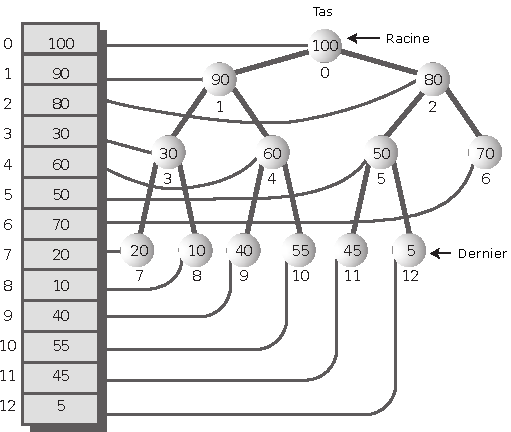
\includegraphics[scale=1]{figs/heap}
\end{figure}
\end{frame}

\begin{frame}{Tas}{TDA file avec priorité}
Un tas convient à l'implémentation d'une file avec priorité :
\begin{itemize}
\item une opération \texttt{int remove()} : retourne le noeud de clé maximum (priorité maximum)
\item une opération \texttt{insert(int key)} d'insertion dans le tas.
\end{itemize}

\end{frame}

\begin{frame}{Tas}{Partiellement ordonnée}
\begin{itemize}
\item $\neq$ ABR : pas de parcours ordonné simple
\item $\neq$ ABR : pas de recherche efficace
\item chaque chemin est ordonné
\item insertion rapide
\item suppression du n\oe ud de clé maximum rapide 
\end{itemize}

\end{frame}

\begin{frame}{Tas}{Suppression}
\hl{Principe}: 
\begin{enumerate}
\item Suppression de la racine
\item Dernier n\oe ud(en bas à droite de l'arbre) placé à la racine
\item Échange avec le plus grand des fils tant que la condition d'ordre n'est pas respectée
\end{enumerate}
\end{frame}

\begin{frame}{Tas}{Suppression}
\begin{figure}
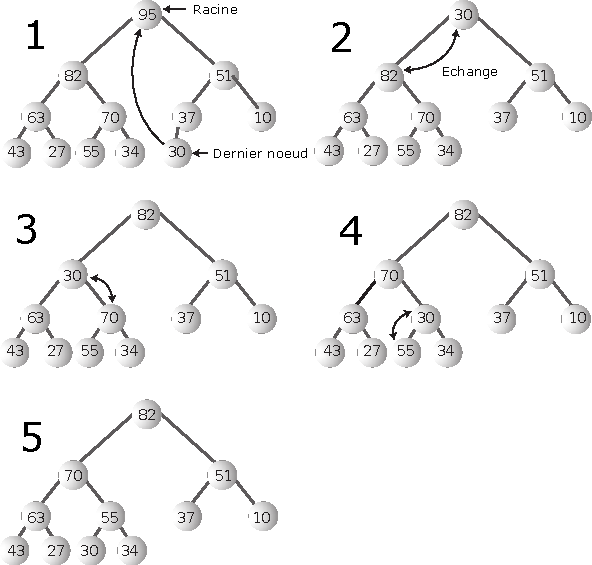
\includegraphics[scale=0.7]{figs/heap_remove}
\end{figure}
\end{frame}

\begin{frame}{Tas}{Insertion}
\hl{Principe}: 
\begin{enumerate}
\item Ajout du n\oe ud en bas à droite
\item Échange avec le père tant que la condition d'ordre n'est pas respectée
\end{enumerate}
\end{frame}

\begin{frame}{Tas}{Insertion}
\begin{figure}
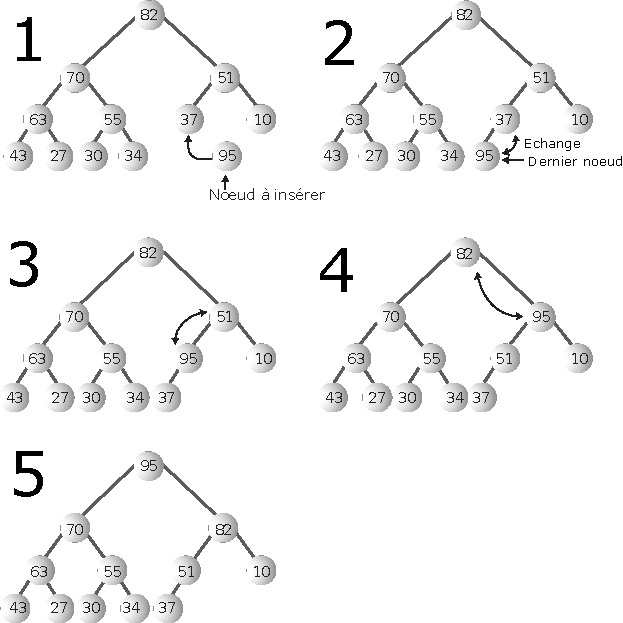
\includegraphics[scale=0.65]{figs/heap_insert}
\end{figure}
\end{frame}


\begin{frame}{Tas}{Tri par tas}
\hl{Principe}: 
Soit un tableau $A$ en entrée :
\begin{enumerate}
\item Insertions successives des valeurs de $A$ dans un tas
\item Suppressions successives sur le tas ajoutées dans un tableau $B$ en partant de la fin de $B$. 
\end{enumerate}
\end{frame}




\end{document}

